\documentclass{book}
\usepackage{polyglossia}  % Hyphenation
\setmainlanguage{english}
\setotherlanguages{french,italian}
\usepackage{minted}       % Source code typesettings
\setminted{breaklines=true}
\usepackage{placeins}     % Float barriers
\usepackage{tikz}         % Diagrams
\usetikzlibrary{trees,arrows}
\usepackage{fancyvrb}     % Manually colored verbatim
\usepackage{float}        % Non-floating figures
\usepackage{url}          % URLs
\usepackage[              % Bibliography
  backend=biber,
  style=alphabetic,
  citestyle=alphabetic,
  sorting=anyt
]{biblatex}
\addbibresource{main.bib}
\usepackage{makeidx}      % Index
\makeindex
\usepackage[nottoc]{tocbibind}
\usepackage{./main}       % Markup and design
% Chapter 1
\defacronym[cite=asa63]{ASCII}{the American Standard Code for Information Interchange}
\defacronym{ASA}{the American Standard Association}
\defacronym{IBM}{the International Business Machines Corporation}
\defacronym{FORTRAN}{the FORmula TRANslator}
\defacronym{COBOL}{the COmmon Business-Oriented Language}
\defacronym{ISO}{the International Organization for Standardization}
\defacronym{IEC}{the International Electrotechnical Commission}
\defacronym[cite=iso93]{UCS}{the Universal multiple-octet coded Character Set}
\defacronym{BMP}{the Basic Multilingual Plane}
\defacronym{UTF}{the \acroshort{UCS} Transformation Format}
\defacronym{BOM}{the Byte Order Mask character}
\defacronym{EBCDIC}{the Extended Binary Coded Decimal Interchange Code}
\defacronym{PC}{the \acroshort{IBM} Personal Computer}
\defacronym{JIS}{the Japanese Industrial Standards encoding}
\defacronym{EUC}{the Extended Unix Code}
\defacronym{SR}{Sound Recognition}
\defacronym{OCR}{Optical Character Recognition}
\defacronym{IME}{Input Method Editor}
\defacronym{GUI}{Graphical User Interface}
\defacronym{CLI}{Command Line Interface}
\defacronym[extra={Also known as the Berkeley Unix}]%
  {BSD}{the Berkeley Software Distribution}
\defacronym{joe}{the Joe's Own Editor}
\defacronym{pico}{the PIne COmposer}
\defacronym{emacs}{the Eventually Munches All Computer Storage editor}
\defacronym{vi}{the Visual Interactive editor}
\defacronym{vim}{\acroshort{vi} IMproved}
\defacronym[short-plural={es}]{DPS}{Document Preparation System}
\defacronym[cite={iso08}]{PDF}{the Portable Document Format}
\defacronym[cite={iso12}]{OOXML}{the Office Open XML format}
\defacronym[cite={iso15}]{ODF}{the Open Document Format for office applications}
% Chapter 2
\defacronym{GML}{the General Markup Language}
\defacronym{SGML}{the Standard General Markup Language}
\defacronym{DTD}{Document Type Declaration}
\defacronym[cite=bray98]{XML}{the eXtensible Markup Language}
\defacronym{Relax NG}{the REgular LAnguage for \acronym{XML} New Generation}
\defacronym[cite=duerst05]{IRI}{the Internationalized Resource Identifier}
\defacronym[cite=lie96]{CSS}{the Cascading Style Sheets language}
\defacronym{TEI}{the Text Encoding Initiative}
\defacronym{MathML}{the Mathematical Markup Language}
\defacronym{SVG}{the Scalable Vector Graphics language}
\defacronym[foreign={\foreign[french]{la Conseil Européen pour la Recherche
  Nucléaire}}]{CERN}{the European Organization for Nuclear Research}
\defacronym{HTML}{the HyperText Markup Language}
\defacronym{W3C}{the World Wide Web Consortium}
\defacronym[cite=pemberton00]{XHTML}{the eXtensible Hypertext Markup Language}
\defacronym[cite=lassira99]{RDF}{the Resource Description Framework}
\defacronym{DC}{the Dublin Core}
\defacronym{FOAF}{Friend Or A Foe}
\defacronym[cite=mcguinness04]{OWL}{the Web Ontology Language}
\defacronym{JSON}{the JavaScript Object Notation}
\defacronym{LD}{Linked Data}
\defacronym[cite=sporny14]{JSON-LD}{\acronym{JSON} for \acronym{LD}}
\defacronym[cite=adida08]{RDFa}{\acronym{RDF} in attributes}
\defacronym{WYSIWYG}{What You See Is What You Get}
\defacronym{GNU}{\acroflat{GNU} is Not Unix}
\defacronym{API}{Application Programming Interface}
\defacronym{ECMA}{the European Computer Manufacturers Association}
\mdefacronym{ATnT}{AT\scamp T}{the American Telephone and Telegraph corporation}
\defacronym{DTP}{DeskTop Publishing}
% Bibliography
\defacronym{USA}{the United States of America}
\defacronym{MA}{Massachusetts}
\defacronym{NY}{New York}
\defacronym{TC}{a Technical Committee}
\defacronym{JTC}{a Joint \acronym{TC}}
\defacronym{SC}{a SubCommittee}
\defacronym{WG}{a Working Group}
\defacronym{RFC}{a Request For Comments}
\defacronym{CA}{California}
\defacronym{CLDR}{the Common Locale Data Repository}
        % Acronyms
\begin{document}

\frontmatter
\title{Electronic Document Preparation\\Pocket Primer}
\author{Vít Novotný}
\maketitle
\tableofcontents
\mainmatter

\fakechapter{Foreword}
With the advent of the digital age, typesetting has become available to
virtually anyone equipped with a personal computer. Beautiful text documents can
now be crafted using free and consumer-grade software, which often obviates the
need for the involvement of a professional designer and typesetter. The level
playing field of the Internet coupled with the rising popularity of digital-only
documents then allows the author to bypass the publisher as well, if they so
wish, without jeopardizing their chance of recognition.

Documents are like tin-cans, conserving ideas for later consumption. This one in
particular contains a number of thoughts that should prove useful for any author
who aspires to write, design, typeset and distribute text documents---the most
universal and common kind of documents in use. Each chapters describes one
discrete step of text document preparation along with the relevant tools and
literature. Since document preparation is a broad, multidisciplinary subject,
the main goal of this text is to provide the reader with a general overview of
the landscape and to present references to more detailed literature for those
interested in further nourishment.

\chapter{Writing}
The essence of a document is the idea it represents. In the case of a text
document, this idea is articulated through speech, which is transcribed using
text, optionally accompanied by figures and then laid out on a sheet of paper
according to a design. Since the text is typically independent on the design,
whose task is to support and elicit the internal structure of the text, it is
writing that is the logical first step in the text document creation.

  % An example of a poem by Christian Morgenstern
  % as an exception to the rule
  % \caption{Exceptions that prove the rule about the separation of text
  %   and design can sometimes be encountered in poetry. Above is Christian
  %   Morgenstern's \work{Trichter}, where the text and its form are intimately
  %   intertwined.}

The essentials of writing in any given natural language include \term{grammar
rules}\index{rules!grammar}, which specify the structure of spoken language, and
\term{orthographic rules}\index{rules!ortography}, which impose additional
requirements on written text. The complexity of either set of rules depends
entirely on the language in question. Some writing systems, such as the Japanese
kanji, are not phonographic and the correspondence between spoken words and
written ideographs needs to be memorized by the writer on a word-to-word
basis. Some languages, such as Czech, use vastly different grammar rules for
speaking and for writing, which means that a spoken sentence needs to be
translated first before writing down. These specifics need to be recognized by
the writer.

On top of grammar and orthographic rules stand \term{style guides}\index{style
guide}, which, in order to improve consistency, codify how common language
patterns are encoded.\footnote{
  This document was prepared in accordance with William Strunk's \work{Elements
  of Style}: an American English style guide for general use.
} More comprehensive style guides---such as \work{the Chicago Manual of Style}
or Ritter's \work{Oxford Style Manual}---often go beyond writing and provide
guidelines on design and typesetting as well, making them an indispensable
reference on the editorial tradition.

Above all stand the \term{typographic rules}\index{rules!typography}, which
specify how the resulting document should be typeset so that it doesn't disturb
the eye of the reader. These, as well as the orthographic rules on hyphenation,
can be safely ignored during writing, for the realm of thought knows no type
areas.

  % An illustration of the journey of an idea from the author to the reader

\section{Text Processing}
Originally the domain of the pen, the quill, the stylus, and the more recent
typewriter machine, manuscripts of today are produced chiefly using the personal
computer. The discipline of creating and manipulating digital text is called
\term{\inx{text processing}} and will be the focus of this section.

\subsection{Character Encoding}
Although computing at its most primal has no use for anything but numbers, it
has nevertheless been accompanied by text from the very outset. Even the
earliest computers from 1950s were programmed with both raw machine code and
the text programming languages of \acronym{FORTRAN} and \acronym{COBOL}. The
digital representation of letters, digits and other characters was initially
closely tied to each specific application and processor architecture, but with
the advent of networking in 1960s, mutual intelligibility became a point of
concern. ``We had over sixty different ways to represent characters in
computers. It was a real Tower of Babel,'' explains in \cite{brandel99}
\person{Bob Berner}, an American computer scientist who worked at \acronym{IBM}
during 1956--1962 and who drafted \acronym{ASCII}---the \term{\inx{character
encoding}}, standardized in \cite{asa63}, that unified the industry and enabled
computer networking on large scale.

\subsubsection{ASCII}
In \acronym{ASCII}, every character is represented by a number from 0 to 127,
which is transformed to a seven-bit integer called \term{a \inx{character
code}}. These 128 codes are used to encode \term{\inx{printable
character}s}---spanning the letters of the English alphabet, digits,
punctuation, and other symbols---and \term{\inx{control code}s}, as depicted in
Table \ref{tab:ascii}. Unlike printable characters, control codes have no fixed
visual representation or precise semantics and were used to implement
application-specific communication protocols and text formatting. Unconstrained
by the bandwidth and the storage limitations of the 1960s, today's communication
protocols and text formats gravitate towards markup constructed from printable
characters, which, unlike control codes, are easy to read and write by humans.

  % The ASCII table (both the original and ANSI X3.4-1986: [tab:ascii]
  %   <http://sliderule.mraiow.com/w/images/7/73/ASCII.pdf>

%%% ASCII, Other Standards
%%%   <https://en.wikipedia.org/wiki/ASCII#Other_standards>
%%%   <https://en.wikipedia.org/wiki/ISO/IEC_8859-2#External_links>
%%%
%%% Character histories: notes on some Ascii code positions
%%%   <http://www.cs.tut.fi/~jkorpela/latin1/ascii-hist.html>
%%%
%%% ASCII: American Standard Code for Information Infiltration
%%%   <http://worldpowersystems.com/J/codes/>
%%%
%%% Encyclopedia of Computer Science, 4th edition
%%%   <https://dl.acm.org/ralston.cfm?CFID=698031209&CFTOKEN=46500462>
%%%
%%% Theoretical Foundation of Regular Expressions and Text Editors
%%%   <http://citeseerx.ist.psu.edu/viewdoc/download?rep=rep1&type=pdf&doi=10.1.1.126.9920>
%%%
%%% A History of Scientific Text Processing at CERN
%%%   <http://ref.web.cern.ch/ref/CERN/CNL/2001/001/tp_history/>
%%%
%%% When and how did text enter the world of computing, eventually to be
%%% standardized as ASCII in 1963? <http://qr.ae/RHFEzE>
%%%
%%% IBM's Early Computers: A Technical History
%%%   <http://www.amazon.com/IBMs-Early-Computers-Technical-Computing/dp/0262523930>

The following properties make it easy to manipulate and reason about character
strings encoded in \acronym{ASCII}:
\begin{itemize}
  \item Each character is represented by exactly seven bits. This makes it easy
    to allocate space for character strings of fixed length, to measure the
    number of characters stored in a memory region, and to perform basic
    operations, such as adjacent character retrieval or text truncation.
  \item Characters are alphabetically ordered. Character strings can therefore
    be collated by the comparison of character code binary values.
  \item Lower-case letters, upper-case letters, digits and control codes form
    contiguous ranges of character codes, which simplifies classification.
  \item There is precisely one way to encode any printable character. The
    conversion between the lower- and upper-case letters is a matter of
    inverting one bit.
\end{itemize}
This comes at the expense of support for non-English writing systems.

\subsubsection{Eight-bit Encodings}
With the byte size stabilizing at eight bits, new character encodings emerged
that were based on \acronym{ASCII} and utilized the additional bit to encode
characters of non-English writing systems. Beside the numerous vendor-specific
encodings (called \term{\inx{codepage}s}), a set of 15 eight-bit encodings
covering all major modern writing systems whose characters fit within the space
of 128 additional combinations was standardized in the
\work{\acroshort{ISO}/\acroshort{IEC} 8859} series released during 1986--2001.

  % An example of the lower 128 bytes of the Latin-2 encoding (with citation)

Compared to \acronym{ASCII}, eight-bit encodings introduced an additional level
of complexity to text processing:
\begin{itemize}
  \item Each character is exactly eight bits wide. The manipulation with strings
    is therefore as straightforward as with \acronym{ASCII}.
  \item Character strings can no longer be collated by character code
    comparison. Each encoding requires a separate mapping from character codes
    to sorting weights.
  \item Classes of characters, such as upper-case letters, lower-case letters,
    and punctuation, no longer form contiguous ranges and their position varies
    among encodings. This impedes character classification.
  \item Idiosyncrasies, such as the ligature of æ and invisible hyphenation
    hints, are included in several encodings, which makes it more difficult to
    determine character string equivalence. Among encodings that contain lower-
    and upper-case letters, the algorithms for case conversion vary.
  \item There exists no standard mechanism to detect which encoding is being
    used. The distinction needs to be done on the application level using either
    heuristics or additional metadata. Consequently, no standard mechanism
    exists to use different character encodings within a single text document.
\end{itemize}
A portion of this complexity is inherent in the task of encoding the characters
of all modern writing systems, but the overhead caused by the character encoding
fragmentation proved to be hurtful and unnecessary.

\subsubsection{The Universal Character Set and Unicode}
The continual increase in the available bandwidth and storage led to the
creation of the competing standards of Unicode \cite{unicode91,unicode92} and
\acronym{UCS} \cite{iso93} in an attempt to create a text encoding that would
contain the characters of all the world's living languages and succeed
\acronym{ASCII} as the \foreign[italian]{lingua franca} of text interchange.

\Acronym{UCS} is an ever-expanding catalogue of characters from writing systems
both modern and ancient, and symbols ranging from diacritical marks,
punctuation, and ideograms to mahjong tiles, alchemical symbols, and the ancient
Greek musical notation. Each of these characters is assigned a number ranging
from 0 to 2,147,483,647 (\hexa{7FFFFFFF}) with the numbers of the most common
characters in the range from 0 to 65,535 (\hexa{FFFF}) called \acronym{BMP}.
\Acronym{UCS} encodings map character numbers to binary character codes. Three
major encodings are specified in the \acronym{UCS} standard and its
amendments \cite{iso93:am1,iso93:am2}:
\begin{description}
  \item[\acroshort{UTF}-32]\acroindex[!UTF-32@{\acroshort{UTF}-32}]{UTF}
    Directly encodes \acronym{UCS} characters by transforming the character
    numbers to four-byte integers. This encoding is also known as
    \acroshort{UCS}-4\acroindex[!UCS-4@{\acroshort{UCS}-4}]{UCS}.
  \item[\acroshort{UTF}-16]\acroindex[!UTF-16@{\acroshort{UTF}-16}]{UTF}
    Directly encodes characters within \acronym{BMP} by transforming the
    character numbers to two-byte integers. Character numbers in the range from
    65,536 to 1,114,111 (\mbox{\hexa{010000}--\hexa{10FFFF}}) are transformed
    into a pair of two-byte integers, called \term{a \inx{surrogate pair}},
    ranging from 55,296 to 57,343 (\mbox{\hexa{DC00}--\hexa{DFFF}}). To enable
    the \acroshort{UTF}-16 encoding, the character numbers in the surrogate pair
    range will never be assigned. The same applies to character numbers greater
    than 1,114,111 (\hexa{10FFFF}), which allows \acroshort{UTF}-16 to encode
    any \acroshort{UCS} character.
  \item[\acroshort{UTF}-8]\acroindex[!UTF-8@{\acroshort{UTF}-8}]{UTF}
    Directly transforms character numbers from 0 to 127 (\hexa{7F}) to one-byte
    integers. Since the beginning of the \acroshort{BMP} matches
    \acronym{ASCII}, any text encoded in eight-bit \acroshort{ASCII} is also
    encoded in \acroshort{UTF}-8. Character numbers in the range from 127 to
    1,114,111 (\mbox{\hexa{00007F}--\hexa{10FFFF}}) are transformed into two to
    four one-byte integers ranging from 128 to 253
    (\mbox{\hexa{80}--\hexa{FD}}). The encoding is illustrated in Figure
    \ref{fig:utf8}.
\end{description}
\acroshort{UTF}-32 is primarily used for the internal representation of
individual \acronym{UCS} characters inside programs. \acroshort{UTF}-16 fulfills
the same role for applications that only work with \acronym{BMP}.
\acroshort{UTF}-8 is used for text storage and interchange; since 2010, the
majority of text content on the Web is encoded in \acroshort{UTF}-8
\cite{qsuccess15}.

  % A table explaining the UTF-8 encoding [fig:utf8]
  % Some examples of exotic glyphs in Unicode

% Unicode > ISO/IEC 10646: Sorting, directionality, how it combines with other
% characters, numeric values <https://en.wikipedia.org/wiki/Universal_Coded_Character_Set#External_links>
%
% Adopce UTF-8: <https://en.wikipedia.org/wiki/UTF-8#/media/File:UnicodeGrow2b.png>
% Standardy UTF-7 a UTF-EBCDIC
%
% UTF-8:  RFC 3629
% UTF-16: RFC 2781
% <https://tools.ietf.org/html/rfc5198> 
%
% Unicode signature: FEFF (byte order mask)
%
% Unicode was initially intended as a 16-bit encoding (leaving out ancient
% scripts, see [[Unicode 88, pages 4--5]])
% UCS was initially intended as a 32-bit encoding (wasn't approved by vendors) => compromise
%
% Příklad možností několika zakódování stejně vypadajících symbolů:
%   <https://en.wikipedia.org/wiki/Number_Forms> (římské číslice), ellipsis,
%   soft hyphen, combination sequences
%
% Unicode and ISO 10646 merged in version 1.1
% The big achievement of Unicode: Unification of ideographic glyphs
%
% Přidat brevity disclaimery ohledně ostatních existujících kódování
%   ISO/IEC 646, EBDIC, Baudot Code, Morse Code
%   14-bitový JIS a odvozená kódování
%   ... [[ASCII: Other Standards]]

%%% Unicode 101: An Introduction to the Unicode Standard
%%%   <http://www.interproinc.com/blog/unicode-101-introduction-unicode-standard>
%%%
%%% Unicode Implementation levels
%%%   <http://www.cl.cam.ac.uk/~mgk25/unicode.html#levels>
%%%
%%% Unification of the Unicode Standard and ISO 10646
%%%   <http://www.unicode.org/versions/Unicode1.0.0/V2ch01.pdf>
%%%
%%% Unicode 88 <http://unicode.org/history/unicode88.pdf>
%%% Unicode equivalence <https://en.wikipedia.org/wiki/Unicode_equivalence>
%%%
%%% Plane (Unicode):
%%%   <https://en.wikipedia.org/wiki/Plane_(Unicode)#Basic_Multilingual_Plane>

\subsection{Text Manipulation}
% Inserting Unicode symbols on Windows, Linux, iOS, Android
\subsection{Revision Control}
\section{Word Processing}

\chapter{Markup}
A manuscript can consist of a seamless river of words and still make perfect
sense to the author. To truly capture its meaning in a clear and unambiguous
manner, however, the manuscript will often need to be supplemented with a set of
annotations. At a more basic level, this refers to the compliance with the
orthographic rules---such as the correct spelling, capitalization, word breaks,
and punctuation---that are specific to the language of the document.  It is not
at all unreasonable to expect that this basic compliance should be already met
by the manuscript. At a higher level, this consists of discovering and marking
up the inner order and logic of the text, so that the resulting document can
later be typeset in a way that visually reflects its structure, and
supplementing the document with additional figures.

\index{markup!logical|(}\index{markup!presentation|(}
To this end, there exists a wealth of \term{markup languages} that enable the
enrichment of text with additional information and labels. Aside from
\term{logical markup}, which captures the logical structure of the document, markup
languages may also provide \term{presentation markup}, which directly impacts
the visual properties of the document but carries no semantic information. The
usage of presentation markup makes it impossible to separate the markup from the
design and to capture the logic of the text. As a result, the consistency in the
design of each logical part of the document needs to be ensured manually, and
future changes of design become error-prone and tedious. In this regard, logical
markup is to design what style guides are to writing: a means of ensuring
consistency that should be used whenever appropriate.
\index{markup!logical|)}\index{markup!presentation|)}

\section{Meta Markup Languages}
\subsection{The General Markup Language}
The situation engulfing digital typesetting was growing increasingly frustrating
for publishers in the 1960s. The markup languages used by different typesetting
systems varied wildly, and once a publisher had a large collection of documents
typeset via a given company, switching to another one could be very costly
venture. The companies would often take advantage of this situation, causing
their prices to skyrocket. As a result of that, a demand for a universal markup
language emerged.

This demand was met by a project developed\footnote{
  More information about the project can be found within the personal
  recollections of its co-author, Charles F. Goldfarb, in \cite{goldfarb96} and
  \cite{goldfarb97:whySGML}.
} at the Cambridge Scientific Center of \acronym{IBM} in the early 1970s. The
project aimed at imbuing a text editor with the ability to query, edit, and
display documents from a repository to allow the usage of computers in legal
practice. Very early on in the development process, it became clear that the
crux was going to be the markup languages in which the documents were written.
These languages were not unified and many of them comprised largely presentation
markup, which made information retrieval impossible without the use of
heuristics. To resolve these issues, a unifying markup language called
\acronym{GML} was drafted. The language was later released to the public in
\cite{goldfarb81} and finally standardized as \acronym{SGML}\footnote{
  The authoritative resource on \acronym{SGML} is \cite{goldfarb91}, which
  includes the full text of the standard along with the author's extensive
  annotations.
} within \cite{iso8879}.

\Acronym{SGML} documents consist of text mixed with \term{tags}%
\acroindex[!tag]{SGML}, which delimit meaningful sections of the document called
\term{elements}\acroindex[!element]{SGML}. Elements can carry additional
information in \term{attributes}\acroindex[!attribute]{SGML}. Additionally,
\acronym{SGML} documents may contain miscellaneous instructions for the program
that is processing it, as well as human-readable comments. Repeated strings of
text can be declared as \term{entities} \acroindex[!entity]{SGML} that can
consequently be used throughout the document in place of the original strings.

Although the described structure is shared by all \acronym{SGML} documents, the
actual syntax, as well as the restrictions with regards to the contents and the
attributes of individual elements, are declared within a \acronym{DTD}, which
can be different for each document. It is worth noting that a \acronym{DTD} only
declares the syntax of an \acroshort{SGML} document; the semantics of the
individual elements and their attributes are left to the interpretation of the
program processing the document. The syntax and the constraints imposed by a
\acronym{DTD} define an \term{application} \acroindex[!application]{SGML} of
\acronym{SGML}. An \acronym{SGML} document is considered to be a valid instance
of an \acroshort{SGML} application, when it conforms to the respective
\acronym{DTD}.

\subsection{The Extensible Markup Language}
Although \acronym{SGML} was designed to be the general format for data exchange,
the complexity of the specification and the lack of support for Unicode proved
to be a major hindrance preventing its wider adoption and tool development. As a
response, \acronym{W3C} published a specification of \acronym{XML} in
\cite{bray98}. Along with the introduction of \acronym{XML}, the
\acroshort{SGML} specification received a technical corrigendum of
\cite{goldfarb97:webSGML}, which turned \acronym{XML} into a proper subset of
\acronym{SGML} restrained by an \acroshort{SGML} \acronym{DTD}.

\begin{figure}
  \inputminted{xml}{examples/02/recipe.xml}
  \caption{An example \acronym{XML} document\filename{recipe.xml}}
  \label{fig:recipe}\bigskip
  \inputminted{dtd}{examples/02/dtdtypes}
  \caption{\acronym{SGML} and \acronym{XML} \acronym{DTD}s can be either linked
    to a document through public and system identifiers, directly embedded in
    a document, both linked to and embedded in a document, or left out
    altogether.}
  \label{fig:recipe-dtd}
\end{figure}
        
This \acronym{DTD} completely fixes the syntax of \acronym{XML} documents, which
makes it possible to differentiate two levels of correctness. Specifically, an
\acronym{XML} document is considered to be \term{well-formed}%
\acroindex[!well-formedness]{XML}, when it conforms to the \acroshort{SGML}
\acronym{DTD} that restrains \acronym{XML} as well as to the additional
constraints given in the specification. An \acroshort{XML} document is
considered to be \term{valid} \acroindex[!validity]{XML} against an
\acroshort{XML} \acronym{DTD}, when it is well-formed and conforms to the said
\acronym{XML} \acronym{DTD}.  Along with \acronym{DTD}s, there exists a wealth
of \term{schema languages}\acroindex[!schema language]{XML}\footnote{
  A list of tools for the manipulation of files in \acronym{XML} schema
  languages is maintained on the web site of \acronym{W3C} at
  \url{http://www.w3.org/XML/Schema}.
} for \acronym{XML}, such as \acroshort{W3C} \acroshort{XML} Schema
\acroindex[!Schema]{XML}, \acronym{Relax NG}, or Schematron that can be used to
check the validity of an \acroshort{XML} document instead of a \acronym{DTD}.
The constrains imposed by either a \acronym{DTD} or a schema define an
\term{application}, \term{language}, or \term{format}
\acroindex[!application]{XML} \acroindex[!language]{XML}
\acroindex[!format]{XML} of \acronym{XML}.

Along with schema languages, other supplementary languages also exist, such as
\inx{XPointer}, \inx{XPath}, and \inx{XQuery} for addressing sets of elements
(fragments) within a \acronym{XML} document or \acronym{CSS} for specifying the
visual properties of an \acroshort{XML} document. Although some of these
languages may not be \acronym{XML} languages, they are nevertheless used within
documents of various \acronym{XML} formats and form an important part of the
ecosystem.

A notable new feature of \acronym{XML} are \term{namespaces}%
\acroindex[!namespace]{XML}, which were added to the specification with the
release of \cite{bray99}. Namespaces enable the inclusion of elements and
attributes of different \acronym{XML} applications within a single \acronym{XML}
document by providing a method to qualify element and attribute names with
\acropl{IRI} that uniquely represent the respective \acronym{XML} applications.
Namespaced elements are a spiritual successor of a more expressive
\acronym{SGML} feature of \inx{\identifier{CONCUR}}, which makes it possible to
mark up several structural views of a single document. Unlike with
\identifier{CONCUR}, which ties each view to an \acroshort{SGML} \acronym{DTD},
there exists no general mechanism for the translation of \acropl{IRI} to
\acronym{XML} schemata.  This makes it impossible to validate namespaced
\acronym{XML} documents, unless all used \acropl{IRI} and their respective
schemata are known to the parser.

\begin{figure}[hb!]
  {\tikzstyle{level 1}=[sibling distance=\baselineskip, level distance=1.5cm]
\begin{tikzpicture}[grow=right]
  \node {\textcolor{red}{Speech}}
    child {
      node [label=right:{AASE: See, you dare not! Every word of it's a
        lie!} ] {}}
    child {
      node[label=right:{PEER: Swear? Why should I?}] {} }
    child {
      node[label=right:{AASE: Well then, swear to me it's true!}] {}}
    child {
      node[label=right:{PEER: No, I'm not!}] {} }
    child {
      node[label=right:{AASE: Peer, you're lying!}] {} };
  \node [below=5\baselineskip] {\textcolor{blue}{Verse}}
    child {
      node[label=right:{Every word of it's a lie!} ] {}}
    child {
      node[label=right:{Swear? Why should I? See, you dare not!}] {} }
    child {
      node[label=right:{Well then, swear to me it's true!}] {}}
    child {
      node[label=right:{Peer, you're lying! No, I'm not!}] {} };
\end{tikzpicture}}%
\begin{Verbatim}[commandchars=\\\{\},codes={\catcode`$=3\catcode`^=7\catcode`_=8}]
<(\textcolor{blue}{V})line>
  <(\textcolor{red}{S})speech who="Aase">Peer, you're lying!</(\textcolor{red}{S})speech>
  <(\textcolor{red}{S})speech who="Peer">No, I'm not!</(\textcolor{red}{S})speech>
</(\textcolor{blue}{V})line><(\textcolor{blue}{V})line>
  <(\textcolor{red}{S})speech who="Aase">Well then,
    swear to me it's true!</(\textcolor{red}{S})speech>
</(\textcolor{blue}{V})line><(\textcolor{blue}{V})line>
  <(\textcolor{red}{S})speech who="Peer">Swear, why should I?</(\textcolor{red}{S})speech>
  <(\textcolor{red}{S})speech who="Aase">See, you dare not!
</(\textcolor{blue}{V})line><(\textcolor{blue}{V})line>
  Every word of it's a lie!</(\textcolor{red}{S})speech>
</(\textcolor{blue}{V})line>
\end{Verbatim}

  \caption{The markup of the dramatic and metrical views of the beginning of
    Henrik Ibsen's \work{Peer Gynt} using the \identifier{CONCUR} feature of
    \acronym{SGML}}
\end{figure}

%%% Živoucí CONCAT <http://webylon.info/K.24>
%%% Popis SGML deklarace pro ISO/IEC15445
%%%   <http://www.angelovic.cz/internet/sgml-deklarace.html#concur>

\begin{figure}[H]
  \inputminted{xml}{examples/02/recipe.xsd}
  \caption{A reformulation of the recipe \acronym{DTD} from Figure
    \ref{fig:recipe-dtd} in the \acroshort{XML} Schema \acroindex[!Schema]{XML}
    language.\filename{recipe.xsd}}
  \label{fig:recipe-xsd}
  \inputminted{text}{examples/02/recipe.rnc}
  \caption{A reformulation of the recipe \acronym{DTD} from Figure
    \ref{fig:recipe-dtd} in the compact syntax of \acronym{Relax NG}.%
    \filename{recipe.rnc}}
  \label{fig:recipe-rnc}
  \inputminted{sh}{examples/02/recipe.sh}
  \caption{\acronym{XML} documents can be easily validated against \acronym{XML}
    schemata using command-line tools, such as \inx{\identifier{xmllint}}.}
\end{figure}

Due to the reduced complexity of \acronym{XML} compared to \acronym{SGML}, the
language was adopted by specialists and the general public alike and has
superseded \acronym{SGML} in many applications. Some of the applications of
\acronym{XML} for document preparation include DocBook\acroindex[!DocBook]{XML}%
\footnote{
  The authoritative resource on the DocBook \acronym{XML} format is
  \cite{walsh10}. The book itself is written in DocBook and its source code is
  publicly available at the Web page at \url{http://docbook.org}.
}---a technical documentation format used for authoring books by publishers such
as O'Reilly Media and for documenting software at companies such as Red Hat,
\acroflat{SuSE}, or Sun Microsystems---, \acronym{TEI}---a general text encoding
format for the use in the academic field of digital humanities---,
\acronym{MathML}---a format for describing mathematical formulae---, or
\acronym{SVG}---a two-dimensional vector image format. Other \acroshort{XML}
applications, such as \acroshort{XHTML} and \acroshort{RDF}/\acroshort{XML}, will
be discussed in Section \ref{sec:www-markup}.
      
\section{Markup on the World Wide Web}\label{sec:www-markup}
\subsection{The Hypertext Markup Language}
In \cite{bernerslee89}, an English computer scientist \person{Timothy John
Berners-Lee} proposed a decentralized system for sharing linked documents within
\acronym{CERN}. The system laid foundation for today's \term{\inx{World Wide
Web}} (Web) and earned its author knighthood.  The markup language used to write
documents for the system was an application of \acronym{SGML} called
\acronym{HTML}. In 1993, the Web started to gain popularity amongst the general
public owing to the release of the first graphical Web browser Mosaic, which
paved way for the Web browsers of today. In 1994, \person{Timothy John
Berners-Lee} formed \acronym{W3C}, which has since been developing the standards
for the Web.

The first standard version of \acronym{HTML} was \acronym{HTML} 2.0 published in
\cite{rfc1866}. As the Web was becoming ubiquitous, it began accumulating an
increasing number of documents that weren't valid instances of \acronym{HTML},
since most Web browsers, when faced with a malformed document, would act in
accordance with the Postel's law and try to render the document despite its
deficiencies. In an attempt to unify the way malformed \acronym{HTML} documents
were rendered across the Web browsers, \acronym{W3C} acknowledged and documented
this behaviour as a part of \cite[Section~8.2, Parsing HTML
documents]{hickson14}. An example is presented in Figure
\ref{fig:overlapping-elements}.

\begin{figure}[b]
  \begin{minted}[linenos]{html}
<b>This text is bold, <i>bold and italic</b>, italic.</i>
<b>This text is bold, </b><i><b>bold and italic</b>, italic.</i>
  \end{minted}
  \caption{The fragment on line 1 contains overlapping elements and, as such, it
    can't be a part of a valid \acronym{HTML} document. Nevertheless, it is
    recommended by \acronym{W3C} that browsers parse the fragment identically to
    the fragment on line 2.}
  \label{fig:overlapping-elements}
\end{figure}

Initially, \acronym{HTML} only comprised a mixture of logical and presentation
markup with fixed visual interpretation. This changed with the specification of
\acronym{CSS}, which was introduced by \acronym{W3C} in \cite{lie96}. The
language enabled the specification of the visual properties of any element,
which allowed for the separation of document markup and design, effectively
eliminating the need for the presentation markup.

\begin{figure}
  \inputminted{html}{examples/02/presentation-markup.html}
  \caption{An excerpt from the Web site of the \acroshort{CSS} Zen Zarden
    located at \protect\url{http://csszengarden.com}. The document above was
    created using the \acroshort{HTML} presentation markup. The document below
    achieves the same appearance by the combination of logical markup and
    \acronym{CSS} definitions.}\bigskip
  \inputminted{html}{examples/02/logical-markup.html}
\end{figure}

During the same period, an initial version of a scripting language called
\inx{JavaScript} was drafted and incorporated into Netscape Navigator 2.0%
\footnote{
  \inx{JScript} and \inx{VBScript} were direct competitors of JavaScript, but
  they never saw implementation outside Microsoft browsers.
} of the contemporary leading web browsers and a descendant of the original
Mosaic browser. As a part of a joint effort to bring Java into web browsers by
Sun Microsystems and Netscape Communications, JavaScript was, according to
\cite{js-announcement}, supposed to complement Java applets -- a role it has
since outgrown. Standardized in \cite{ecma1}, JavaScript blurs the line between
static documents and interactive applications and remains the predominant
client-side programming language for the Web. Since, however, the support of
JavaScript by a Web browser is fully optional, it is considered a good practice
to use it chiefly for the enrichment of already self-sufficient \acronym{HTML}
documents. In case of an interactive application, this recommendation can be
relaxed.

\subsection{The Extensible Hypertext Markup Language}
Ever since the release of \acronym{XML} in 1998, \acronym{W3C} entertained the
idea of turning \acronym{HTML} into an application of \acronym{XML}, rather than
\acronym{SGML}, as exemplified by the working draft of \cite{raggett98}. Unlike
\acronym{HTML} parsers, which are complex in their acceptance of malformed
content, \acronym{XML} parsers are, as per \cite[Section~1.2,
Terminology]{bray98}, required to draconianly refuse \acronym{XML} documents
that aren't well-formed, leading to architectural simplicity and decreased
computational requirements. As a result, reformulating \acronym{HTML} in
\acronym{XML} was suggested as a way to bring the Web to mobile, embedded, and
other devices limited in their resources, as well as to reduce the amount of
malformed documents on the Web in general. Other perceived advantages included
the ability to use \acronym{XML} tools for web documents and to include
instances of other \acronym{XML} applications, such as \acronym{MathML} and
\acronym{SVG}, directly into web documents using \acronym{XML} namespaces.

The idea was brought to fruition in \cite{pemberton00} as an \acronym{XML}
application named \acronym{XHTML}. \acronym{XHTML} was met with lukewarm
reception, since many of its supposed benefits proved to be either questionable
or too marginal to warrant migration from \acronym{HTML}. The speed advantages
of the simpler parser were largely offset by its lack of support for incremental
rendering, caused by the impossibility to validate partially downloaded pages,
the closing of the gap in the computing power between mobile and desktop devices
made it possible to use full-fledged \acronym{HTML} parsers across the spectrum,
and the lack of ways to provide alternative content for browsers that would not
support directly included \acroshort{XML} documents considerably reduced the
usefulness of \acronym{XML} namespaces. As a result, \acronym{XHTML} has yet to
succeed in replacing \acronym{HTML} and remains an alternative markup language
for the Web.

%%% Content-Negotiation Techniques to serve XHTML as text/html and
%%% application/xhtml+xml
%%%   <http://www.w3.org/2003/01/xhtml-mimetype/content-negotiation>

\subsection{The Semantic Web and Linked Data}
The underlying fundament of the Web is the the idea of a globally available and
incrementally scalable base of human knowledge. \acronym{HTML} and
\acronym{XHTML} succeeded in fulfilling this vision for human-readable documents
but didn't provide a unifying machine-readable format for the representation of
structured information that would enable the creation of a web of linked data
running in parallel to the web of documents. To remedy that, \acronym{W3C}
released \cite{lassira99} containing the specification of \acronym{RDF}, a
method for the description of resources on the Web.

Drawing from the research in the field of knowledge representation, an
\acroshort{RDF} document represents data as a set of \term{triples}%
\acroindex[!triple]{RDF}. Each of the triplets comprises \term{a
predicate}\acroindex[!predicate]{RDF}, \term{a
subject}\acroindex[!subject]{RDF}, and \term{an object}\acroindex[!object]{RDF},
where both the predicate and the subject are specified as \term{resources}
\acroindex[!resource]{RDF} using \acropl{IRI}. If the object of a triplet
$(p,s,o)$ is also a resource, the triplet can be interpreted as a subject $s$
being in a relation $p$ with the object $o$. If the object is a \term{literal
value} \acroindex[!literal]{RDF} rather than a resource, the triplet can be
interpreted as a subject $s$ having a property $p$ with the value $o$.

Resources in \acronym{RDF} are specified via \acropl{IRI} to prevent naming
collisions in \acronym{RDF} documents created independently by distinct authors.
These \acropl{IRI} are not required to resolve to an actual web page, and
disregarding the small set of standard resources specified within the
\acroshort{RDF} specification, they carry no inherent meaning. In order to
describe a set of resources, the relationships between them, and their intended
meaning in an \acroshort{RDF} document, an extension of the set of standard
resources---called \acroshort{RDF} Schema and specified in
\cite{brickley04}---can be used. The resulting documents are called
\term{ontologies} \acroindex[!ontology]{RDF} and can be used for automated
reasoning about \acronym{RDF} documents containing resources described by the
ontology.\footnote{
  A list of ontologies that are fully documented, honor the current best
  practices, and are supported by various tools can be found on the
  \acroshort{W3C} wiki at \url{http://www.w3.org/wiki/Good_Ontologies}.
} Some of the well-known ontologies include \acronym{DC}---an ontology for the
generic description of both web multimedia and physical objects---,
\acronym{FOAF}---an ontology for the description of people and their social
relationships---, or the Music Ontology---an ontology for the description of
entities related to the music industry, such as albums, artists, tracks, and
events. More expressive standards for the creation of ontologies, such as
\acronym{OWL} specified in \cite{mcguinness04}, also exist.

The syntax of \acronym{RDF} is not fixed, meaning that, beside the
\acroshort{XML} serialization specified in \cite{lassira99}, other languages,
such as \acronym{JSON-LD} specified in \cite{sporny14}, the \inx{Turtle}
language specified in \cite{beckett14:turtle}, or the line-based \inx{N-Triples}
language specified in \cite{beckett14:nt}, can be used to represent an
\acroshort{RDF} document. A noteworthy serialization of \acronym{RDF} is
\acronym{RDFa} specified in \cite{adida08}. Although various serializations of
\acronym{RDF} can be included in or linked to an \acroshort{HTML} or
\acroshort{XHTML} document, this will often result in an undesirable duplication
of data already present in the document. To prevent this, \acronym{RDFa}
utilizes the content already present within the underlying \acroshort{HTML} or
\acroshort{XHTML} document using element attributes. The usage of \acronym{RDF}
in conjunction with \acronym{HTML} and \acronym{XHTML} is intended to gradually
obsolete the loosely-defined use of \acronym{CSS} class names, attributes, the
\element{meta} element, and the \element{link} element to encode additional
application-specific metadata about the document---a technique known as
\term{microformatting}.

\begin{figure}
  \inputminted{xml}{examples/02/john.rd}
  \inputminted{text}{examples/02/john.nt}
  \inputminted{text}{examples/02/john.ttl}
  \caption{Above is an example \acronym{RDF} document using \acronym{DC} and
    \acronym{FOAF} ontologies in \acronym{RDF}/\acronym{XML}%
    \filename{john.rd}, \inx{N-Triples}\filename{john.nt}, and \inx{Turtle}%
    \filename{john.ttl} serializations. Below is a graph representation of the
    document.}\label{fig:rdf-doc}\bigskip
  {\tikzstyle{level 1}=[sibling distance=6\baselineskip, level distance=0.5cm]
\tikzstyle{level 2}=[sibling distance=6\baselineskip, level distance=0.5cm]
\centerline{\begin{tikzpicture}[grow=right,->]
  \node[label=left:{\url{http://example.org/document.html}}] {}
    child { node {\texttt{"The Web page of John Smith"@en}}
      edge from parent
      node[left] {\textcolor{blue}{dc:title}}}
    child { node {\url{http://example.org/john-smith}}
      child { node[label=right:{foaf:Person}] {}
        edge from parent
        node[right,align=left] {\textcolor{blue}{rdf:type}}}
      child { node {\texttt{"John Smith"}}
        edge from parent
        node[left] {\textcolor{blue}{foaf:name}}}
      edge from parent
      node[left] {\textcolor{blue}{foaf:creator}};
    };
\end{tikzpicture}}}

\end{figure}

\begin{figure}[t!]
  \inputminted{html}{examples/02/john.html.linked-rdf}
  \caption{Above is an \acroshort{HTML} document linked to the \acroshort{RDF}
    document from Figure \ref{fig:rdf-doc}. Below is the same \acroshort{HTML}
    document with the \acroshort{RDF} data directly embedded using the
    \acroshort{RDFa} serialization.}\bigskip
  \inputminted{html}{examples/02/john.html.rdfa}
\end{figure}

%%% Linked Data
%%%   <http://www.w3.org/DesignIssues/LinkedData.html>
%%%
%%% Tim Berners-Lee: The next web
%%%   <http://www.ted.com/talks/tim_berners_lee_on_the_next_web>
%%%
%%% The SPARQL Query Language for RDF (SPARQL) and the (at the time of
%%% writing only drafted) Linked Data Fragments RDF query interfaces
%%%   <http://www.w3.org/TR/rdf-sparql-query/>
%%%   <http://linkeddatafragments.org/specification/>
%%%
%%% The Rule Interchange Format (RIF)
%%%   <http://www.w3.org/TR/rif-overview/>
        
\section{Markup in Document Preparation Systems}
Some of the existing markup is directly tied with specific document preparation
systems. These can be dichotomized into \term{batch-oriented systems}
\index{document preparation system!batch-oriented}, which process marked up input
text documents into printable output documents in a page description language on
demand, and \term{interactive systems} \index{document preparation
system!interactive}, which allow the user to directly edit an approximation of
the output document via a visual editor. Also called \acronym{WYSIWYG},
interactive systems exchange mild learning curve for more primitive typesetting
algorithms that don't stand in the way of interactivity and for reduced
flexibility stemming from the usage of a \acronym{GUI}, which, although often
intuitive for simple tasks, seldom matches the power of the markup languages
used by batch-oriented systems.

\subsection{Batch-oriented Document Preparation Systems}
One of the archetypal batch-oriented systems are \inx{\identifier{troff}}, whose
function is to produce output for general printers, and \identifier{nroff}%
\index{\identifier{nroff}|seealso{\identifier{troff}}}, whose function is to
produce output for line printers and text terminals. Both tools were developed
as a proprietary software for the Unix operating system at the beginning of
1970s by \acronym{ATnT}. An alternative to \identifier{nroff} and
\identifier{troff} is
\identifier{groff}\index{\identifier{groff}|seealso{\identifier{troff}}}, which
was developed as a free software in 1980 by \acronym{GNU}. \Identifier{groff}
combines the capabilities of both tools and is still used extensively for the
markup of documentation in Unix and Unix-like operating systems, although more
advanced alternatives for general typesetting (such as \TeX) exist. The
associated markup language combines presentation markup with programming
constructs and allows the definition of logical markup in the form of user
macros. Standard macro packages, such as \inx{\identifier{man}} for the
formatting of documentation, \identifier{me}
\index{\identifier{troff}!\identifier{me}} for the creation of research papers,
or the more recent \identifier{mom} \index{\identifier{troff}!\identifier{mom}}
for general typesetting tasks are typically distributed along with the system.
Special markup invokes preprocessors that can be used for the typesetting of
tables, equations, and vector graphics.

\begin{figure}
  \fbox{\includegraphics[clip,trim=1.7cm 12cm 1.7cm 1.3cm,%
    width=0.975\textwidth]{examples/02/poe-groff.pdf}}
  \inputminted{groff}{examples/02/poe.groff}
  \caption{An excerpt from the beginning of Edgar Allen Poe's \work{Cask of
    Amontillado} formatted using the \identifier{mom}
  \index{\identifier{troff}!\identifier{mom}} macro package of
  \inx{\identifier{groff}}.}
  \label{fig:poe}
\end{figure}

%%% The Groff and Friends HOWTO
%%%   <http://troff.org/TheGroffFriendsHowto.pdf>
%%%
%%% Writing Macros
%%%   <https://www.gnu.org/software/groff/manual/html_node/Writing-Macros.html>
%%%
%%% A User's Guide to the Lout Document Formatting System
%%%   <https://www.urz.uni-heidelberg.de/imperia/md/content/urz/programme/text/lout.pdf>

Another notable batch-oriented system is \TeX\index{TeX@\TeX}\footnote{
  The circumstances that led to the creation of \TeX\ and the surrounding tools
  are thoroughly documented in \cite{knuth98}.
}, which was developed and consequently released to the public domain in 1970s
by an American professor of computer science \person{Donald Knuth}, after he had
received galley proofs for the second volume of his monograph, \work{the Art of
Computer Programming}, and found the appearance of mathematical formulae
distasteful.  As a result, the typesetting of mathematics is a central theme in
\TeX, rather than an afterthought, which differentiates it from most other
document preparation systems and which largely contributed to the massive
popularity \TeX\ has attained in academia. Much like in the case of
\identifier{troff} and its derivatives, the language of \TeX\ is ripe with
typographic and programming primitives and doesn't by itself contain logical
markup. The language, however, allows for the creation of user macros. An
example of a macro package that makes it possible to create documents of various
classes with pure logical markup is \inx{\LaTeX}: the standard markup language
for academic and technical documents.

\begin{figure}
  \inputminted{tex}{examples/02/poe.tex}
  \caption{The \identifier{groff} document from Figure \ref{fig:poe}
    reformulated using \TeX}
\end{figure}

\subsection{Interactive Document Preparation Systems}
Interactive systems come in two distinctive flavours. \emph{Word processors}
\index{document preparation system!interactive!word procesing} are
the digital progeny of the typewriter machine, with which they share the main
function of fast text capture. The typewriter output documents served largely as
a manuscript for designers and typographers, who then produced the actual
published work. With the advent of personal computing and the Web,
self-publishing became more approachable to the general public, and modern word
processors can be used not only to write but also to design and typeset
documents, although the offered functionally is typically constrained by user
experience demands. This concern is not shared by \emph{desktop publishing
software}\index{document preparation system!interactive!desktop publishing},
which provides refined control over the resulting page layout and the
typesetting primitives. The ability to produce document comparable to those set
using traditional typography comes at the expense of steeper learning curve.

Most interactive systems will provide a means to mark up sections of text.
Presentation markup performs direct changes of typographic properties, such as
the face, family, variant, color, or the size of the font that is used to
typeset the text. Logical markup enables the classification of sections of text
with the ability to set up the design of each class later on. This decouples
writing and markup from design and makes it easy to change the design of the
entire document and difficult to produce inconsistent design.

\begin{figure}
  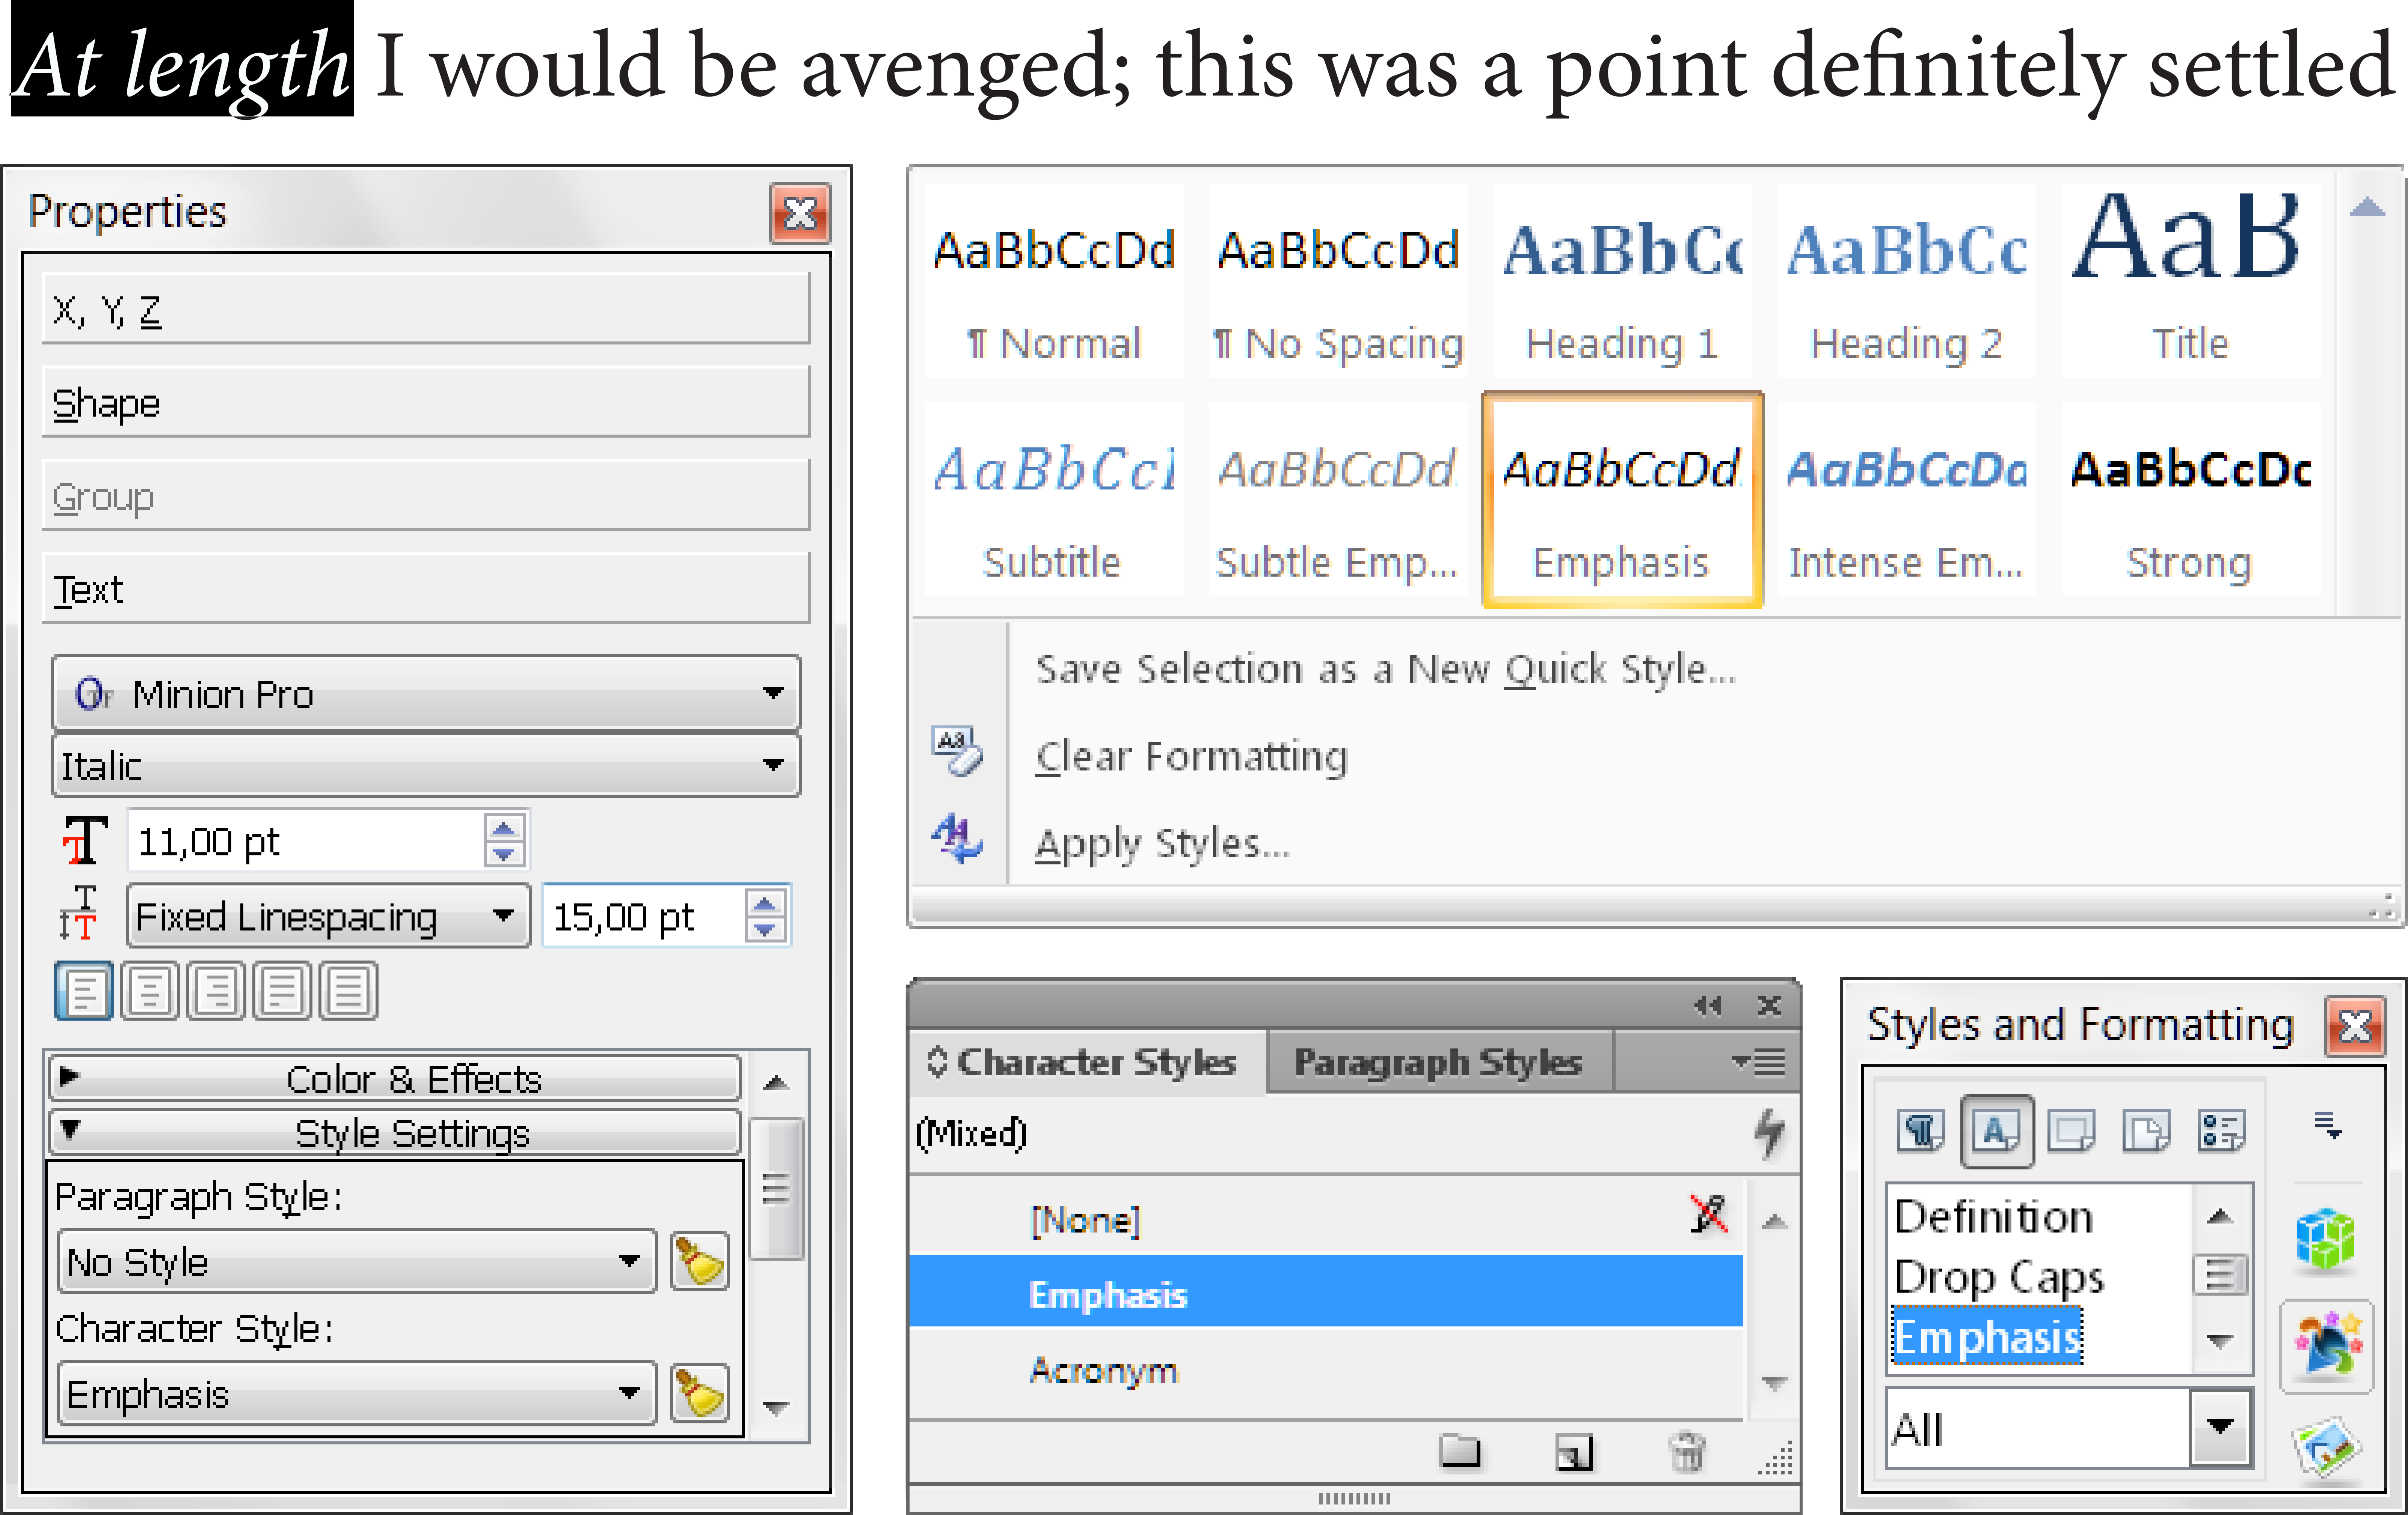
\includegraphics[width=\textwidth]{examples/02/interactive-editors.png}
  \caption{Logical markup in the interactive document preparation systems of
    \inx{Scribus} (left), \inx{Microsoft Word} (above), \inx{Adobe InDesign}
    (below left) and \inx{Apache OpenOffice} (below right)}
\end{figure}

\section{Lightweight Markup Languages}
Parallel to the heavy-duty applications of \acronym{SGML} and \acronym{XML},
there runs a vein of markup languages that give priority to unobtrusiveness and
legibility over expressiveness and genericity. Rooted in the reality of
computer text terminals with limited formatting capabilities, \term{lightweight
markup languages} \index{lightweight markup language} leverage punctuation and
indentation to produce comparatively weak and domain-specific, but also humane,
highly intuitive, and often profoundly beautiful markup that is easy to both
read and write. Examples of lightweight markup languages include \inx{Markdown},
\inx{Creole}, \inx{AsciiDoc}, \inx{MakeDoc}, \inx{Setext}, or \inx{Wikicode}.
Lightweight markup languages are typically supplemented by tools that enable
the conversion to more general languages such as \acronym{HTML}. Also typical
is the existence of numerous flavours of every lightweight markup language,
which represent different use cases.

\chapter{Design}
% XML -- CSS, XSL, XSLT
\chapter{Typesetting}
% Accessibility -- WCAG
% Digital Typesetting Pocket Primer, Ron Goldberg
% Word processors do offer typographic primitives
%   <http://word.tips.net/T001081_Inserting_a_Non-Breaking_Space.html>
%   Unicode characters:
%     * \hexa{FEFF} -- \unichar{Zero width no-break space}
%     * \hexa{00A0} -- \unichar{Non-breaking space}
%     * \hexa{200B} -- \unichar{Zero width space}
%     * \hexa{0020} -- \unichar{Space}
%     * \hexa{2009} -- \unichar{Thin space}
%     * ... <http://www.fileformat.info/info/unicode/category/Zs/list.htm>
%     * ... <http://www.fileformat.info/search/google.htm?q=zero+width&domains=www.fileformat.info&sitesearch=www.fileformat.info&client=pub-6975096118196151&forid=1&channel=1657057343&ie=UTF-8&oe=UTF-8&cof=GALT%3A%23008000%3BGL%3A1%3BDIV%3A%23336699%3BVLC%3A663399%3BAH%3Acenter%3BBGC%3AFFFFFF%3BLBGC%3A336699%3BALC%3A0000FF%3BLC%3A0000FF%3BT%3A000000%3BGFNT%3A0000FF%3BGIMP%3A0000FF%3BFORID%3A11&hl=en>
%     * ... <http://www.unicode.org/versions/Unicode1.0.0/V2ch01.pdf>, page 6
%
%%% Hyphenation in HTML
%%%   <http://www.cs.tut.fi/~jkorpela/shy.html>
%%%   <https://developer.mozilla.org/en-US/docs/Web/CSS/hyphens>
\chapter{Proofreading}
\chapter{Printing}
\chapter{Distribution}

% Bibliography
\cleardoublepage
\printbibliography[heading=bibintoc]

% Acronyms
\cleardoublepage
\fakechapter{Acronyms}
\printacronyms[heading=none]

% Index
\def\index#1{} % Disable indexing
\printindex    % Print the index
\faketoc{Index}

\end{document}
